\documentclass[12pt, oneside]{article}
\usepackage[letterpaper, margin=1in, headsep=0.5in, left=0.3in, right=2.5in]{geometry}
\usepackage[english]{babel}
\usepackage[utf8]{inputenc}
\usepackage{amsmath}
\usepackage{amsfonts}
\usepackage{amssymb}
\usepackage{tikz}
\usepackage{yhmath}
\usetikzlibrary{quotes, angles}
\usepackage{graphicx}
\usepackage{enumitem}
\usepackage{multicol}

\newif\ifmeta
\metatrue %print standards and topics tags

\title{Regents Geometry}
\author{Chris Huson}
\date{May 2022}

\usepackage{fancyhdr}
\pagestyle{fancy}
\fancyhf{}
\renewcommand{\headrulewidth}{0pt} % disable the underline of the header
\raggedbottom

%\fancyhead[LE]{\thepage}
\fancyhead[RO]{Name:}
\fancyhead[LO]{BECA / Dr. Huson / Geometry Regents - Sorted Problem Bank}
\cfoot{\thepage}

\begin{document}
\subsubsection*{Angle calculation situations}
\begin{enumerate}[itemsep=0cm]
\item In the diagram below, $\overline{FAD} \parallel \overline{EHC}$, and $\overline{ABH}$ and $\overline{BC}$ are drawn.
\begin{center}
  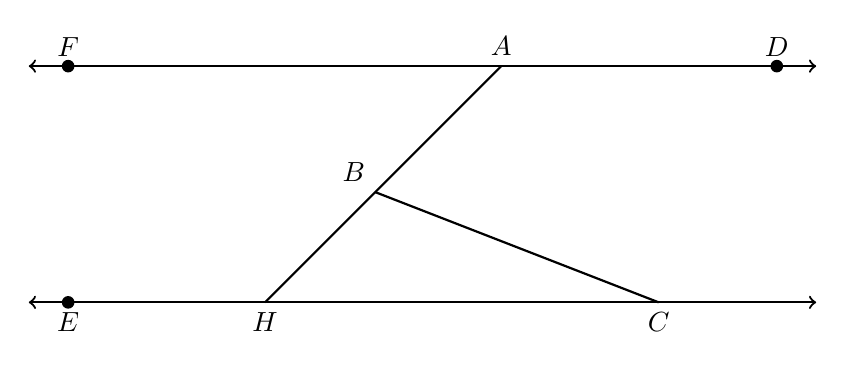
\begin{tikzpicture}[scale=1]
    \draw [thick, <->] (0,0)--(10,0);
    \draw [thick, <->] (0,3)--(10,3);
    \draw [thick] (3,0)node[below]{$H$}--(6,3)node[above]{$A$};
    \draw [thick] (4.4,1.4)node[above left]{$B$}--(8,0)node[below]{$C$};
    \fill (0.5,0) circle [radius=0.08]node[below]{$E$};
    \fill (0.5,3) circle [radius=0.08]node[above]{$F$};
    \fill (9.5,3) circle [radius=0.08]node[above]{$D$};
  \end{tikzpicture}
  \end{center}
If $m\angle FAB = 48^\circ$ and $m\angle ECB = 18^\circ$, what is $m\angle ABC$?
\begin{multicols}{2}
  \begin{enumerate}
    \item $18^\circ$
    \item $48^\circ$
    \item $66^\circ$
    \item $114^\circ$
  \end{enumerate}
\end{multicols}

\item In the diagram below, $\overline{AEFB} \parallel \overline{CGD}$, and $\overline{GE}$ and $\overline{GF}$ are drawn.
\begin{center}
  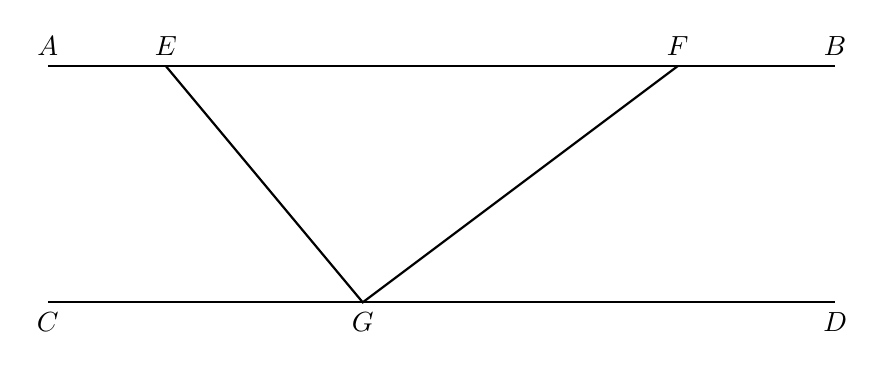
\begin{tikzpicture}[scale=1]
    \draw [thick] (0,0)node[below]{$C$}--(10,0)node[below]{$D$};
    \draw [thick] (0,3)node[above]{$A$}--(10,3)node[above]{$B$};
    \draw [thick] 
      (1.5,3)node[above]{$E$}--
      (4,0)node[below]{$G$}--
      (8,3)node[above]{$F$};
  \end{tikzpicture}
  \end{center}
If $m\angle EFG = 32^\circ$ and $m\angle AEG = 137^\circ$, what is $m\angle EGF$?
\begin{multicols}{2}
  \begin{enumerate}
    \item $11^\circ$
    \item $43^\circ$
    \item $75^\circ$
    \item $105^\circ$
  \end{enumerate}
\end{multicols}

\newpage
\item In the diagram below, $\overline{AB} \parallel \overline{DEF}$, $\overline{AB}$ and $\overline{BD}$ intersect at $C$, $m\angle B = 43^\circ$, and $m\angle CEF = 152^\circ$.
\begin{center}
  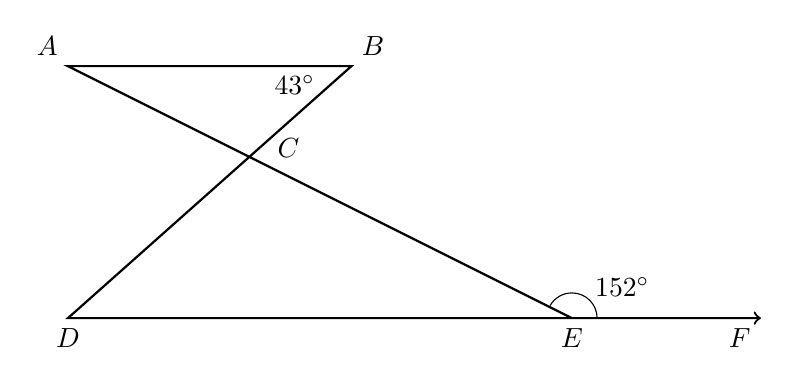
\begin{tikzpicture}[scale=0.8]
    \draw [->, thick] 
      (0,0)node[below]{$E$}--
      (-8,4)node[above left]{$A$}--
      (-3.5,4)node[above right]{$B$}--
      (-8,0)node[below]{$D$}--
      (3,0)node[below left]{$F$};
    \node at (-4.5, 2.7){$C$};
    \node at (-4.4, 3.7){$43^\circ$};
    \node at (0.8, 0.5){$152^\circ$};
    \draw (0.4,0) arc (0:150:0.4);
  \end{tikzpicture}
  \end{center}
Which statement is true?
\begin{multicols}{2}
  \begin{enumerate}
    \item $m\angle D = 28^\circ$
    \item $m\angle A = 43^\circ$
    \item $m\angle ACD = 71^\circ$
    \item $m\angle BCE = 109^\circ$
  \end{enumerate}
\end{multicols}

\item In  $\triangle ABC$ shown below, side $\overline{AC}$ is extended to point $D$ with $m\angle DAB=(180-2x)^\circ$, $m\angle C=(x-10)^\circ$, and $m\angle B=(3x+10)^\circ$.
    \begin{center}
      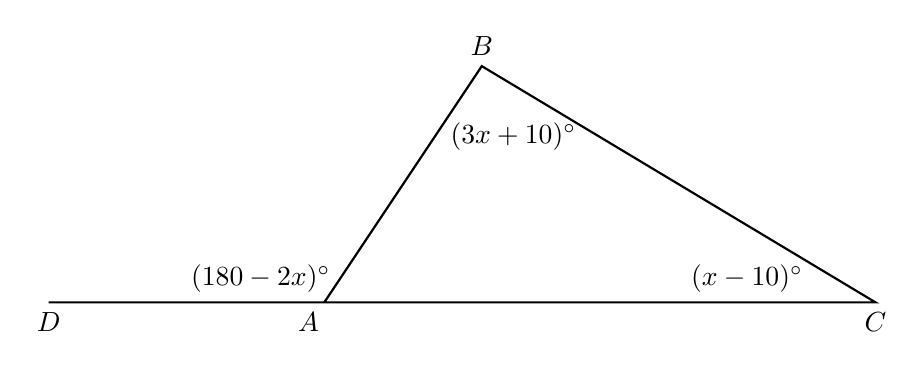
\begin{tikzpicture}
        \draw [thick](-1.5,0)node[below]{$D$}--
          (1.8,0)node[below]{$A$}--
          (9,0)node[below]{$C$}--
          (4,3)node[above]{$B$} --(2,0);
          \node at (2.2,0)[above left]{$(180-2x)^\circ$};
          \node at (8.2,0)[above left]{$(x-10)^\circ$};
          \node at (4.4,2.4)[below]{$(3x+10)^\circ$};
      \end{tikzpicture}
    \end{center}
    What is $m\angle BAC$?

\item In the diagram below of triangle $ABC$, $\overline{AC}$ is extended through point $C$ to point $D$, and $\overline{BE}$ is drawn to $\overline{AC}$.
  \begin{center}
    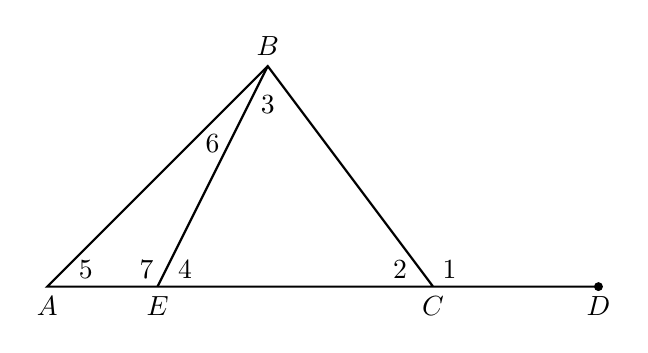
\begin{tikzpicture}[scale=0.7]
    \draw [thick]
    (10,0)node[below]{$D$}--
    (0,0)node[below]{$A$}--
    (4,4)node[above]{$B$}--
    (7,0)node[below]{$C$};
    \draw [fill] (10,0) circle [radius=0.07];
    \draw [thick](2,0)node[below]{$E$}--(4,4);
    \node at (0.7,0.3){5};
    \node at (1.8,0.3){7};
    \node at (2.5,0.3){4};
    \node at (6.4,0.3){2};
    \node at (7.3,0.3){1};
    \node at (3.0,2.6){6};
    \node at (4,3.3){3};
  \end{tikzpicture}
  \end{center}
Which equation is always true?
\begin{multicols}{2}
  \begin{enumerate}
    \item $\angle 1 = m\angle 3 + m\angle 2$
    \item $\angle 5 = m\angle 3 - m\angle 2$ 
    \item $\angle 6 = m\angle 3 - m\angle 2$
    \item $\angle 7 = m\angle 3 + m\angle 2$
  \end{enumerate}
\end{multicols}

\item In diagram of quadrilateral $NAVY$, $m\angle YNA = 30^\circ$, $m\angle YAN = 38^\circ$,\\ $m\angle AVY = 94^\circ$, and $m\angle VAY = 46^\circ$.
\begin{center}
  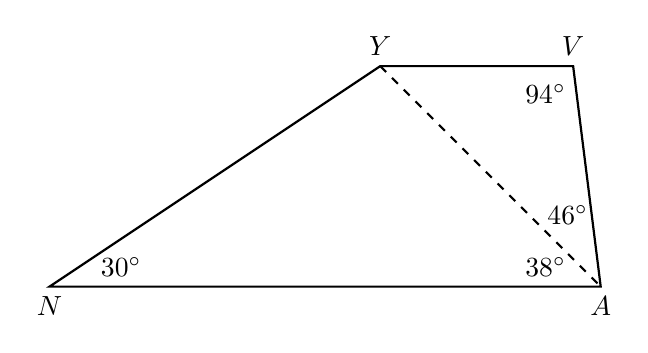
\begin{tikzpicture}[scale=0.7]
    \draw [thick] 
      (0,0)node[below]{$N$}--
      (10,0)node[below]{$A$}--
      (9.5,4)node[above]{$V$}--
      (6,4)node[above]{$Y$}--cycle;
    \draw [dashed, thick] (6,4)--(10,0);
    \node at (1.3,0.35){$30^\circ$};
    \node at (9,0.35){$38^\circ$};
    \node at (9.4,1.3){$46^\circ$};
    \node at (9,3.5){$94^\circ$};
  \end{tikzpicture}
  \end{center}
Which segment has the shortest length?
  \begin{multicols}{2}
  \begin{enumerate}
    \item $\overline{AY}$
    \item $\overline{NY}$
    \item $\overline{VA}$
    \item $\overline{VY}$
  \end{enumerate}
  \end{multicols}

\subsubsection*{Congruence and similarity situations}
\item Triangle $A'B'C'$ is the image of triangle $ABC$ after a translation of 2 units to the right and 3 units up. Is triangle $ABC$ congruent to triangle $A'B'C'$? Explain why.
  
\item In triangle $MAH$ below, $\overline{MT}$ is the perpendicular bisector of $\overline{AH}$.
  \begin{center}
    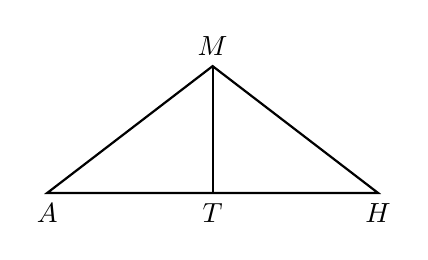
\begin{tikzpicture}[scale=0.7]
    \draw [thick]
    (0,0)node[below]{$A$}--
    (6,0)node[below]{$H$}--
    (3,2.3)node[above]{$M$}--cycle;
    \draw [thick](3,0)node[below]{$T$}--(3,2.3);
  \end{tikzpicture}
  \end{center}
Which statement is \emph{not} always true?
  \begin{enumerate}
    \item $\triangle MAH$ is isosceles.
    \item $\triangle MAT$ is isosceles.
    \item $\overline{MT}$ bisects $\angle AMH$.
    \item $\angle A$ and $\angle TMH$ are complementary.
  \end{enumerate}

\item In the diagram below of circle $O$, points $K$, $A$, $T$, $I$, and $E$ are on the circle, $\triangle KAE$ and $\triangle ITE$ are drawn, $\wideparen{KE} \cong \wideparen{EI}$, and $\angle EKA \cong \angle EIT$.
\begin{center}
  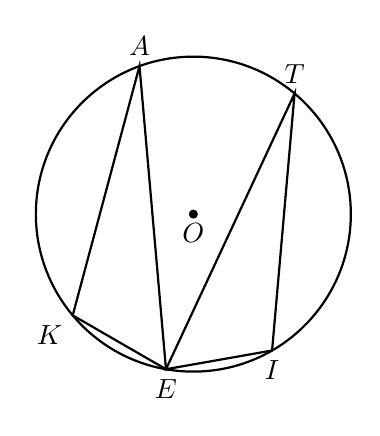
\begin{tikzpicture}[scale=1, rotate=0]
    \draw [fill] (0,0) circle [radius=0.05] node[below]{$O$};
    \draw [thick](0,0) circle [radius=2];
    \draw [thick] 
      (110:2)node[above]{$A$}--
      (220:2)node[below left]{$K$}--
      (-100:2)node[below]{$E$}--cycle;
    \draw [thick] 
      (50:2)node[above]{$T$}--
      (-60:2)node[below]{$I$}--
      (-100:2)--cycle;
  \end{tikzpicture}
  \end{center}
  Which statement about $\triangle KAE$ and $\triangle ITE$ is always true?
  \begin{enumerate}
    \item They are neither congruent nor similar.
    \item They are similar but not congruent.
    \item They are right triangles.
    \item They are congruent.
  \end{enumerate}

\newpage
\subsubsection*{Linear equations}
\item Determine and state an equation of the line perpendicular to the line\\ $5x-4y=10$ and passing through the point $(5,12)$.

\item Write an equation of the line that is parallel to the line whose equation is $3y+7=2x$ and passes through the point $(2,6)$.

\item What is an equation of the image of the line $\displaystyle y=\frac{3}{2}x-4$ after a dilation of a scale factor of $\displaystyle \frac{3}{4}$ centered at the origin?

\item Which equation represents a line that is perpendicular to the line represented by\\[0.25cm] $\displaystyle y=\frac{2}{3}x+1$?
  \begin{multicols}{2}
    \begin{enumerate}
      \item $3x+2y=12$
      \item $3x-2y=12$ 
      \item $\displaystyle y=\frac{3}{2}x+2$
      \item $\displaystyle y=-\frac{2}{3}x+4$
    \end{enumerate}
  \end{multicols}

\item What is an equation of the line that passes through the point $(6,8)$ and is perpendicular to a line with equation $y=\frac{3}{2}x+5$?
  \begin{multicols}{2}
    \begin{enumerate}
      \item $y-8=\frac{3}{2}(x-6)$
      \item $y-8=-\frac{3}{2}(x-6)$ 
      \item $y+8=\frac{3}{2}(x+6)$
      \item $y+8=-\frac{3}{2}(x+6)$
    \end{enumerate}
  \end{multicols}

\item Line $MN$ is dilated by a scale factor of 2 centered at the point $(0,6)$. If $\overline{MN}$ is represented by $y=-3x+6$, which equation can represent $\overline{M'N'}$, the image of $\overline{MN}$?
  \begin{multicols}{2}
    \begin{enumerate}
      \item $y=-3x+12$
      \item $y=-3x+6$ 
      \item $y=-6x+12$
      \item $y=-6x+6$
    \end{enumerate}
  \end{multicols}

\item The line represented by $2y=x+8$ is dilated by a scale factor of $k$ centered at the origin, such that the image of the line has an equation of $y - \frac{1}{2} x=2$. What is the scale factor?
  
\newpage
\subsubsection*{Partition line segments by a given ratio}
\item The endpoints of directed line segment $PQ$ have coordinates of
$P(-7,-5)$ and $Q(5,3)$. What are the coordinates of point $A$, on $\overline{PQ}$, that divide $\overline{PQ}$ into a ratio of 1:3?

\item Point $M$ divides $\overline{AB}$ so that $AM:MB = 1:2$. If $A$ has coordinates $(-1,-3)$ and $B$ has coordinates $(8,9)$, what are the coordinates of $M$?

\item The coordinates of the endpoints of directed line segment $ABC$ are $A(-8,7)$ and $C(7,-13)$. If $AB:BC = 3:2$, what are the coordinates of $B$?

\item Directed line segment $DE$ has endpoints $D(-4, -2)$ and $E(1,8)$.
Point $F$ divides such that $DF:FE$ is $2:3$. What are the coordinates
of $F$?

\newpage
\subsubsection*{Volume, density}
\item A cone has a volume of $108\pi$ and a base diameter of 12. What is the
height of the cone?

\item A child's tent can be modeled as a pyramid with a square base whose sides measure 60 inches and whose height measures 84 inches. What
is the volume of the tent, to the \emph{nearest cubic foot}?

\item Lou has a solid clay brick in the shape of a rectangular prism with a length of 8 inches, a width of 3.5 inches, and a height of 2.25 inches. If the clay weighs 1.055 oz/in$^3$, how much does Lou's brick weigh, to the nearest ounce? 

\item A rectangular tabletop will be made of maple wood that weighs 43 pounds per cubic foot. The tabletop will have a length of eight feet, a width of three feet, and a thickness of one inch. Determine and state the weight of the tabletop, in pounds.

\item The base of a pyramid is a rectangle with a width of 4.6 cm and a
length of 9 cm. What is the height, in centimeters, of the pyramid if
its volume is 82.8 cm$^3$?

\item Randy's basketball is in the shape of a sphere with a maximum circumference of 29.5 inches. Determine and state the volume of the basketball, to the \emph{nearest cubic inch}.

\item As shown in the diagram below, the radius of a cone is 2.5 cm and its slant height is 6.5 cm.
  \begin{center}
    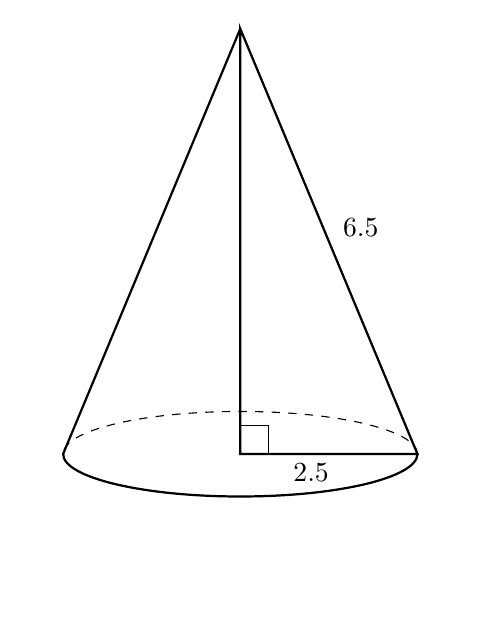
\begin{tikzpicture}[scale=0.9]
    \draw [thick] (0,0)--(2.5,0)--(0,6)--cycle;
    \draw (0,0)++(0.4,0)--++(0,0.4)--+(-0.4,0);
    \draw [thick] (0,6)--(-2.5,0);
    \node at (1,0)[below]{$2.5$};
    \node at (1.7,3.2){$6.5$};
    \draw [dashed] (0,0) ellipse [x radius=2.5,y radius=0.6];
    \clip (-3,-2) rectangle (3,0);
    \draw [thick] (0,0) ellipse [x radius=2.5,y radius=0.6];
  \end{tikzpicture}
  \end{center}
How many cubic centimeters are in the volume of the cone? Express your answer in terms of $\pi$.


\subsubsection*{3-D rotation}
\item Which three-dimensional figure will result when a rectangle 6 inches long and 5 inches wide is continuously rotated about the longer side?
\begin{enumerate}
  \item a rectangular prism with a length of 6 inches, width of 6 inches, and height of 5 inches
  \item a rectangular prism with a length of 6 inches, width of 5 inches, and height of 5 inches
  \item a cylinder with a radius of 5 inches and a height of 6 inches
  \item a cylinder with a radius of 6 inches and a height of 5 inches
\end{enumerate}

\item An isosceles right triangle whose legs measure 6 is continuously rotated about one of its legs to form a three-dimensional object. The three-dimensional object is a
  \begin{enumerate}
    \item cylinder with a diameter of 6
    \item cylinder with a diameter of 12
    \item cone with a diameter of 6
    \item cone with a diameter of 12
  \end{enumerate}

\item Circle $O$ is centered at the origin. In the diagram below, a quarter of circle $O$ is graphed.
  \begin{center}
    \begin{tikzpicture}[scale=0.6]
      %\draw [help lines] (-4,-4) grid (4,4);
      \draw [thick, <->] (-4,0) -- (4,0) node [below right] {$x$};
      \draw [thick, <->] (0,-3)--(0,3) node [left] {$y$};
      %\draw (0,0) circle [radius=2];
      \draw [thick] (-2,0) arc (180:270:2);
      \node at (0,0) [above right]{$O$};
    \end{tikzpicture}
    \end{center}
  Which three-dimensional figure is generated when the quarter circle is continuously rotated about the $y$-axis?
  \begin{multicols}{2}
    \begin{enumerate}
    \item cone
    \item sphere
    \item cylinder
    \item hemisphere
    \end{enumerate}
  \end{multicols}

\item A student has a rectangular postcard that he folds in half lengthwise. Next, he rotates it continuously about the folded edge. Which three dimensional object below is generated by this rotation?
  \begin{multicols}{2}
  \begin{enumerate}
    \item cone
    \item pyramid
    \item cylinder
    \item rectangular prism
  \end{enumerate}
  \includegraphics[scale=0.5]{solids.png}
  \end{multicols}

\item If a rectangle is continuously rotated around one of its sides, what is the three-dimensional figure formed?
  \begin{multicols}{2}
  \begin{enumerate}
    \item cone
    \item sphere
    \item cylinder
    \item rectangular prism
  \end{enumerate}
\end{multicols}

\item If an equilateral triangle is continuously rotated around one of its medians, which 3-dimensional object is generated?
    \begin{enumerate}
      \item cone
      \item sphere
      \item pyramid
      \item prism
    \end{enumerate}

\subsubsection*{Scale effects}
\item After a dilation with center $(0,0)$, the image of $\overline{DB}$ is $\overline{D'B'}$. If $DB=4.5$ and $D'B'=18$, then what is the scale factor of this dilation?

\item Given square $RSTV$, where $RS=9$ cm. If square $RSTV$ is dilated by a scale factor of 3 about a given center, what is the perimeter, in centimeters, of the image of $RSTV$ after the dilation?

\item Jaden is comparing two cones. The radius of the base of cone A is
twice as large as the radius of the base of cone B. The height of cone
B is twice the height of cone A. The volume of cone A is
\begin{enumerate}
  \item twice the volume of cone $B$
  \item four times the volume of cone $B$
  \item equal to the volume of cone $B$
  \item equal to half the volume of cone $B$
\end{enumerate}


\newpage
\subsubsection*{Transformations (onto)}
\item A regular hexagon is rotated about its center. Which degree measure will carry the regular hexagon onto itself? 
\begin{multicols}{2}
  \begin{enumerate}
    \item $45^\circ$
    \item $90^\circ$
    \item $120^\circ$
    \item $135^\circ$
  \end{enumerate}
\end{multicols}

\item What is the smallest non-zero angle of rotation about its center that would map the pentagon onto itself? \vspace{0.25cm} %$ABCDE$
  \begin{center}
      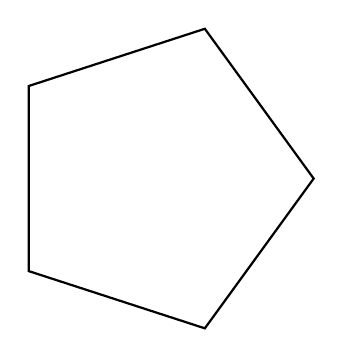
\begin{tikzpicture}%[scale=.48]
        \draw [thick]
        (0:2)--% node[right] {$A$}--
        (72:2)--% node[above right] {$B$}--
        (144:2)--% node[above left] {$C$} --
        (216:2)--% node[left] {$D$}--
        (288:2)--cycle;% node[right] {$E$}--cycle;
      \end{tikzpicture}
    \end{center}

\item Circle YES or NO to indicate whether the given transformation maps the hexagon onto itself.
\vspace{0.5cm}
\begin{multicols}{2}
  \begin{enumerate}
    \item Yes \quad No \quad A reflection over $\overleftrightarrow{AD}$
    \item Yes \quad No \quad A rotation of $60^\circ$ clockwise around the hexagon's center.
    \item Yes \quad No \quad A reflection over a line through the midpoints of  $\overline{BC}$, $\overline{EF}$.
    \item Yes \quad No \quad A rotation of $120^\circ$ counterclockwise around point $D$.
    \end{enumerate}
  \begin{center}
      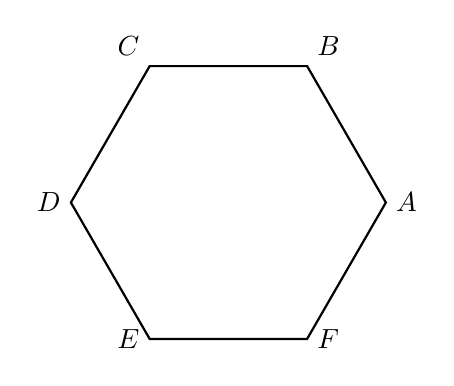
\begin{tikzpicture}%[scale=.48]
        \draw [thick]
        (0:2)node[right] {$A$}--
        (60:2)node[above right] {$B$}--
        (120:2)node[above left] {$C$} --
        (180:2)node[left] {$D$}--
        (240:2)node[left] {$E$}--
        (300:2)node[right] {$F$}--cycle;
      \end{tikzpicture}
    \end{center}
  \end{multicols}

\item The figure shows a rectangle (not a square).
  \begin{center}
    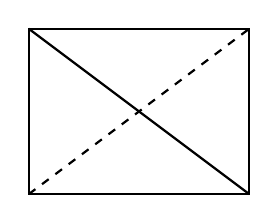
\begin{tikzpicture}[scale=0.7]
      \coordinate (A) at (0, 0); %[label=above left:$P$]
      \coordinate (B) at (4, 0);
      \coordinate (C) at (4, 3);
      \coordinate (D) at (0, 3);
      \draw [thick] (A)--(B)--(C)--(D)--cycle;
      \draw [thick, dashed] (A)--(C);
      \draw [thick] (B)--(D);
      %\draw [thick, xshift=2cm, yshift=2.5cm] (85:3);
    \end{tikzpicture}
  \end{center}
  Which transformations carries the rectangle onto itself? Mark each True or False.
    \begin{enumerate}
      \item A reflection over the solid diagonal \hfill True \quad False
      \item A reflection over the dashed diagonal \hfill True \quad False
      \item A clockwise rotation of $90^\circ$ about the intersection of the diagonals \hfill True \quad False
      \item A clockwise rotation of $180^\circ$ about the intersection of the diagonals \hfill True \quad False
    \end{enumerate}

\item The figure below shows a rhombus with noncongruent diagonals.
  \begin{center}
    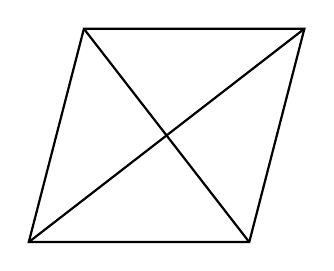
\begin{tikzpicture}[scale=0.7]
      \coordinate (A) at (0, 0); %[label=above left:$P$]
      \coordinate (B) at (4, 0);
      \coordinate (C) at (5, 3.87);
      \coordinate (D) at (1, 3.87);
      \draw [thick] (A)--(B)--(C)--(D)--cycle;
      \draw [thick] (A)--(C);
      \draw [thick] (B)--(D);
      %\draw [thick, xshift=2cm, yshift=2.5cm] (85:3);
    \end{tikzpicture}
  \end{center}
  Which transformation would \emph{not} carry this rhombus onto itself?
    \begin{enumerate}
      \item a reflection over the shorter diagonal
      \item a reflection over the longer diagonal
      \item a clockwise rotation of $90^\circ$ about the intersection of the
      diagonals
      \item a counterclockwise rotation of $180^\circ$ about the intersection of the
      diagonals
    \end{enumerate}
  
\subsubsection*{Sector area and arc length}
\item The diagram below shows circle $O$ with radii $\overline{OA}$ and $\overline{OB}$. The measure of angle $AOB$ is $120^\circ$, and the length of a radius is 6 inches.
\begin{center}
  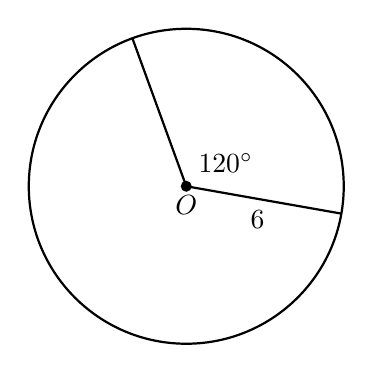
\begin{tikzpicture}[scale=1, rotate=0]
    \draw [thick] (110:2)--(0,0)--(-10:2);
    \draw [thick](0,0) circle [radius=2];
    \fill (0,0) circle [radius=0.07] node[below]{$O$};
    \node at (0.5,0.3){$120^\circ$};
    \node at (-25:1){$6$};
  \end{tikzpicture}
  \end{center}
  Which expression represents the length of arc $AB$, in inches?
  \begin{multicols}{2}
    \begin{enumerate}
      \item $\displaystyle \frac{120}{360}(6\pi)$
      \item $\displaystyle 120(6)$
      \item $\displaystyle \frac{1}{3}(36\pi)$
      \item $\displaystyle \frac{1}{3}(12\pi)$
    \end{enumerate}
  \end{multicols}

\item The area of a sector of a circle with a radius measuring 15 cm is $75\pi \; \rm{cm}^2$. What is the measure of the central angle that forms the sector?

\item A circle with a diameter of 10 cm and a central angle of $30^\circ$ is drawn below.
\begin{center}
  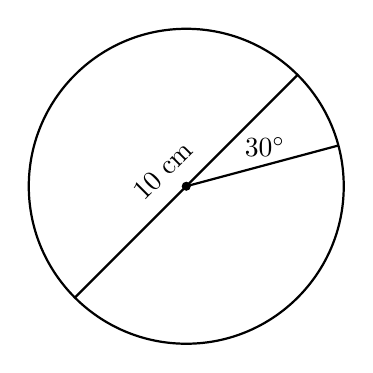
\begin{tikzpicture}[scale=1, rotate=0]
    \draw [thick](0,0) circle [radius=2];
    \draw [thick] (45:2)--(225:2);
    \draw [thick] (0,0)--(15:2);
    \draw [fill] (0,0) circle [radius=0.05];
    \node at (1,0.5){$30^\circ$};
    \node at (-0.3,0.2)[rotate=45]{$10 \; \rm{cm}$};
  \end{tikzpicture}
  \end{center}
  What is the area, to the \emph{nearest tenth of a square centimeter}, of the sector formed by the $30^\circ$ angle?

\item In circle $B$ below, diameter $\overline{RT}$, radius $\overline{BE}$, and chord $\overline{RE}$ are drawn.
\begin{center}
  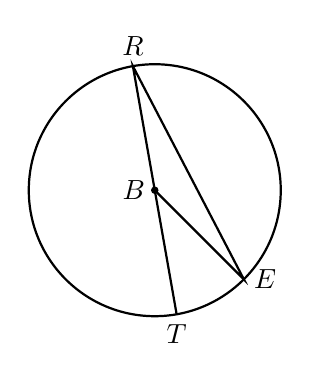
\begin{tikzpicture}[scale=0.8, rotate=0]
    \draw [thick] (0,0)--(100:2)node[above]{$R$}--
    (-45:2)node[right]{$E$}--cycle;
    \draw [thick] (0,0)--(-80:2)node[below]{$T$};
    \draw [fill] (0,0) circle [radius=0.05] node[left]{$B$};
    \draw [thick](0,0) circle [radius=2];
  \end{tikzpicture}
  \end{center}
  It $m\angle TRE = 15^\circ$ and $BE=9$, then the area of sector $EBR$ is what in terms of $\pi$?

\newpage
\subsubsection*{Similar triangles (dilation)}
\item Triangle $JGR$ is similar to triangle $MST$. Which statement is \emph{not}
always true?
\begin{multicols}{2}
  \begin{enumerate}
    \item $\angle J \cong \angle M$
    \item $\angle G \cong \angle T$ 
    \item $\angle R \cong \angle T$
    \item $\angle G \cong \angle S$
  \end{enumerate}
\end{multicols}

\item Given $\triangle ABC \sim \triangle DEF$, $m\angle A=55^\circ$, and $m\angle B=95^\circ$. Find $m\angle E$. \vspace{1cm}

\item In the diagram below $\triangle ABC \sim \triangle DEF$, $DE=10$, $AB=x$, $AC=3x$, $DF=2x+14$. \\[0.25cm] 
Determine the length of $\overline{AB}$.
  \begin{center}
    \begin{tikzpicture}[scale=1]
    \coordinate [label=above left:$A$](A) at (85:2);
    \coordinate [label=below:$B$](B) at (0, 0);
    \coordinate [label=right:$C$](C) at (-20:3);
      \draw [thick] (A)--(B)--(C)--cycle;
      \node at (95:1)[left]{$x$};
      \node at (35:1.75)[right]{$3x$};
      \draw [thick, xshift=5cm, yshift=0.5cm] (85:3) node[above]{$D$}--
      (0,0) node[below]{$E$}--
      (-20:4.5) node[right]{$F$}--cycle;
      \draw [thick, xshift=5cm, yshift=0.5cm](90:1.5) node[left]{$10$};
      \draw [thick, xshift=5cm, yshift=0.5cm](30:2.75) node[right]{$2x+14$};
  \end{tikzpicture}
  \end{center}

\item In the diagram below, $\triangle ABC$ with sides of 10, 13, and 16, is mapped onto $\triangle DEF$ after a clockwise rotation of $90^\circ$ about point $P$. \\*[0.25cm]
  If $DE=3x+1$, what is the value of $x$? 
      \begin{flushright}
        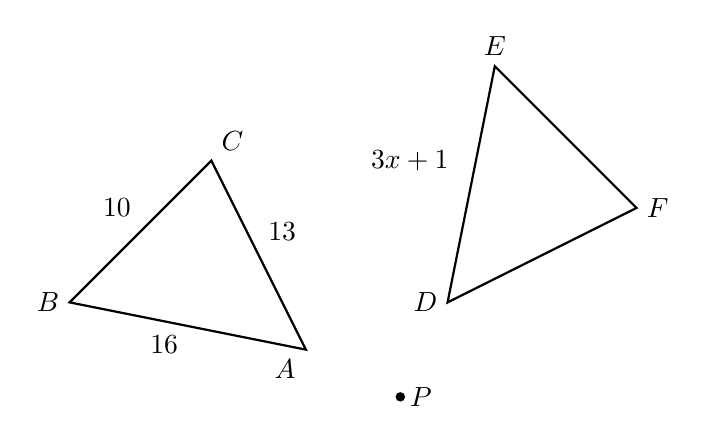
\begin{tikzpicture}[scale=.6]
          %\draw [thick, <->] (-7.4,0) -- (10.4,0) node [right] {$x$};
          %draw [thick, <->] (0,-5.4)--(0,10.4) node [above] {$y$};
          \fill (0,0) circle[radius=0.1] node[right]{$P$};
          \draw [thick]
            (-2,1) node[below left] {$A$}--
            (-7,2) node[left] {$B$}--
            (-4,5) node[above right] {$C$}--cycle;
            \node at (-5,1.5)[below]{16};
            \node at (-6,4){10};
            \node at (-2.5,3.5){13};
            \node at (0.2,5){$3x+1$};
          \draw [thick]
            (1,2) node[left] {$D$}--
            (2,7) node[above] {$E$}--
            (5,4) node[right] {$F$}--cycle;
        \end{tikzpicture}
      \end{flushright}

\item In the diagram below of right triangle $AED$, $\overline{BC} \parallel \overline{DE}$.
  \begin{center}
    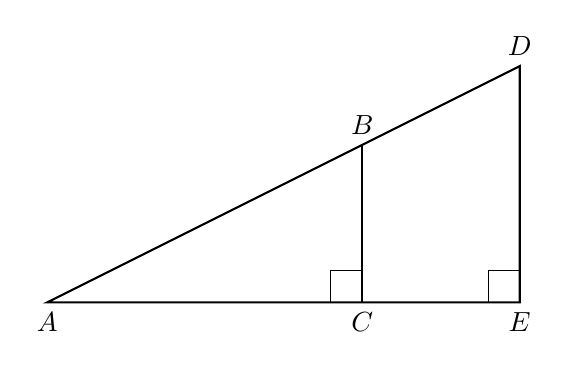
\begin{tikzpicture}[scale=1]
      \draw [-, thick] (0,0) node[below]{$A$}--
      (6,0) node[below]{$E$}--
      (6,3) node[above]{$D$}--cycle;
      \draw [thick] (4,0) node[below]{$C$}--
      (4,2) node[above]{$B$};
      \draw (4,0) ++(-0.4,0)--++(0,0.4)--++(0.4,0);
      \draw (6,0) ++(-0.4,0)--++(0,0.4)--++(0.4,0);
    \end{tikzpicture}
  \end{center} 
  Which statement is always true?
  \begin{multicols}{2}
    \begin{enumerate}[itemsep=0.25cm]
      \item $\displaystyle \frac{AC}{BC} = \frac{DE}{AE}$
      \item $\displaystyle \frac{AB}{AD} = \frac{BC}{DE}$ 
      \item $\displaystyle \frac{AC}{CE} = \frac{BC}{DE}$
      \item $\displaystyle \frac{DE}{BC} = \frac{DB}{AB}$
    \end{enumerate}
  \end{multicols}

\newpage
\item Triangle $ABC$ is dilated with a scale factor of $k$ centered at $A$, yielding $\triangle ADE$, as shown. Given $AB=10$, $BC=14$, $AC=16$, and $DE=21$. Find $CE$.
  \begin{center}
    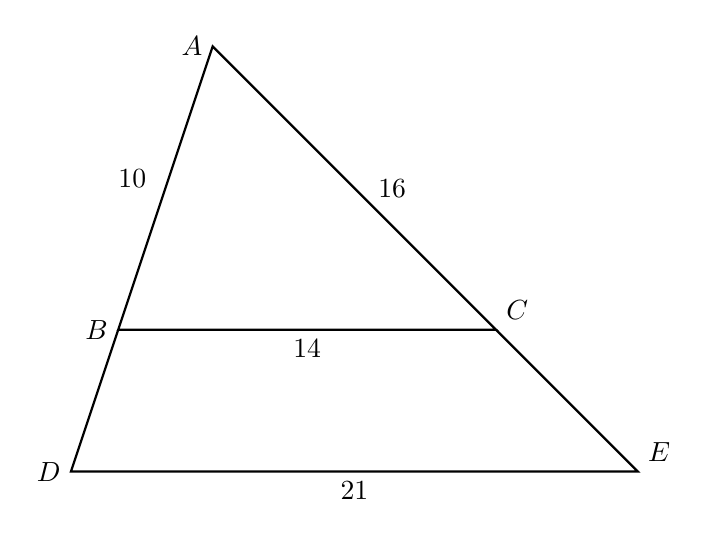
\begin{tikzpicture}[scale=0.6]
      \draw [thick]
      (0,0)node[left]{$B$}--
      (8,0)node[above right]{$C$}--
      (2,6)node[left]{$A$}--cycle;
      \draw [thick]
      (0,0)--
      (-1,-3)node[left]{$D$}--
      (11,-3)node[above right]{$E$}--(8,0);
      \node at (4,0)[below]{$14$};
      \node at (5.3, 3)[right]{$16$};
      \node at (0.3, 2.8)[above]{$10$};
      \node at (5,-3)[below]{$21$};
    \end{tikzpicture}
  \end{center}
  
\item In triangle $ABC$, points $D$ and $E$ are on sides of $\overline{AB}$ and $\overline{BC}$, respectively, such that $\overline{DE} \parallel \overline{AC}$, and $BD:DA = 5:3$.\\[0.5cm]
If $DB=9.0$ and $DE=10.5$, what is the length of $\overline{AC}$, to the \emph{nearest tenth}?
\begin{flushright}
  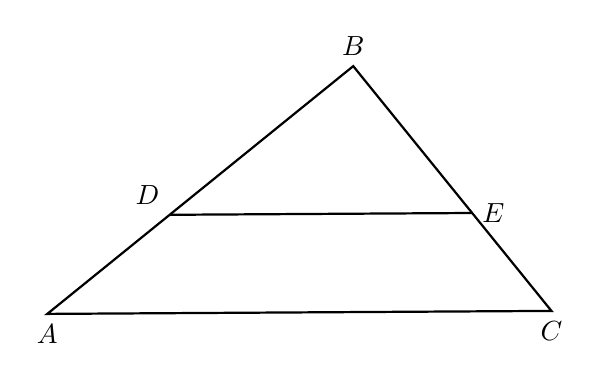
\begin{tikzpicture}[scale=0.5, rotate=-11]
    \draw [thick]
    (0,0)node[above]{$B$}--
    (-130:10)node[below]{$A$}--
    (-40:8)node[below]{$C$}--cycle;
    \draw [thick]
    (-130:6)node[above left]{$D$}--
    (-40:4.8)node[right]{$E$};
  \end{tikzpicture}
\end{flushright}

\item In the diagram below of $\triangle RST$, $L$ is a point on $\overline{RS}$, and $M$ is a point on $\overline{RT}$, such that $\overline{LM} \parallel \overline{ST}$.
\begin{center}
\begin{tikzpicture}[scale=0.7]
  \draw [thick]
  (0,0) node[below] {$R$}--
  (45:10) node[above right] {$T$}--
  (4,0) node[below] {$S$}--cycle;
  \draw [thick]
  (45:2.5) node[above] {$M$}--
  (1,0) node[below] {$L$};
\end{tikzpicture}
\end{center}
If $RL=2$, $LS=6$, $LM=4$, and $ST=x+2$, what is the length of $\overline{ST}$?

\item In the diagram of $\triangle ABC$ below, points $D$ and $E$ are on sides $\overline{AB}$ and $\overline{CB}$ respectively, such that $\overline{DE} \parallel \overline{AC}$.
\begin{center}
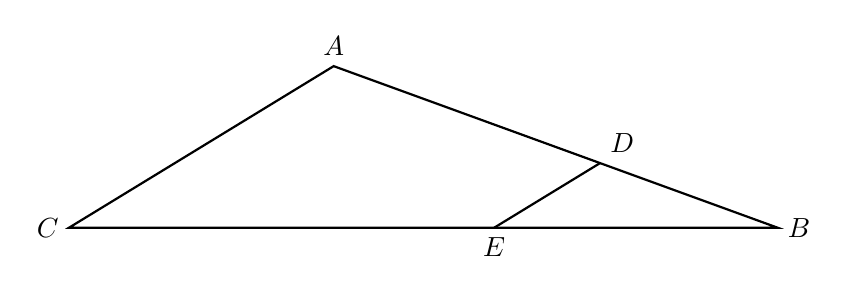
\begin{tikzpicture}[scale=0.6]
  \draw [thick]
  (0,0) node[right] {$B$}--
  (160:10) node[above] {$A$}--
  (-15,0) node[left] {$C$}--cycle;
  \draw [thick]
  (160:4) node[above right] {$D$}--
  (-6,0) node[below] {$E$};
\end{tikzpicture}
\end{center}
IF $EB$ is 3 more than $DB$, $AB=14$, and $CB=21$, what is the length of $\overline{AD}$?

\item Given $\triangle ABP \sim \triangle JKP$ as shown below. $AB=9.6$, $AP=12.0$, $BP=6.3$, and $JP=27.0$. Find $JK$.
  \begin{flushright}
  \begin{tikzpicture}[scale=1.4]
      \draw [thick]
        (-0.25,-1)node[below left]{$B$}--
        (0.5,2)node[left]{$K$}--
        (4,0)node[below left]{$J$}--
        (0,0)node[above left]{$P$}--
        (-2,0)node[left]{$A$}--cycle;
    \end{tikzpicture}
    \end{flushright}

\item In the diagram below, $\overline{AF}$ and $\overline{DB}$ intersect at $C$, and $\overline{AD}$ and $\overline{FBE}$ are drawn such that $\textup{m}\angle D = 65^\circ$, $\textup{m}\angle CBE = 115^\circ$, $DC=7.2$, $AC=9.6$, and $FC=21.6$.
  \begin{center}
  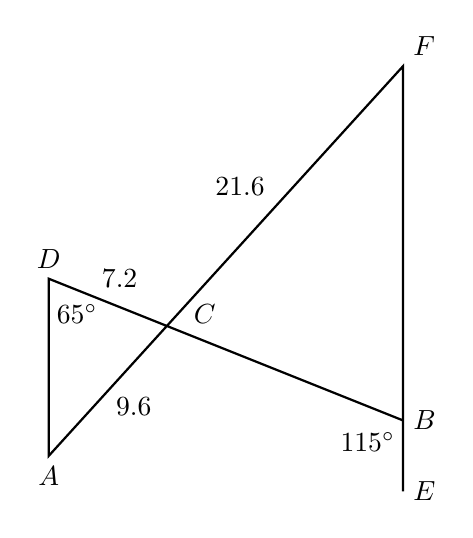
\begin{tikzpicture}[scale=0.9]
    \draw [thick]
      (0,0)node[right]{$B$}--
      (-5,2)node[above]{$D$}--
      (-5,-0.5)node[below]{$A$}--
      (0,5)node[above right]{$F$}--
      (0,-1)node[right]{$E$};
      \node at (-2.8,1.5){$C$};
      \node at (-0.5, -0.3){$115^\circ$};
      \node at (-4.6, 1.5){$65^\circ$};
      \node at (-4, 2){$7.2$};
      \node at (-3.8, 0.2){$9.6$};
      \node at (-2.3, 3.3){$21.6$};
  \end{tikzpicture}
  \end{center}
  What is the length of $\overline{CB}$?


\item In $\triangle ABC$ shown below, $\angle ACB$ is a right angle, $E$ is a point on $\overline{AC}$, and $\overline{ED}$ is drawn perpendicular to hypotenuse $\overline{AB}$.
\begin{center}
  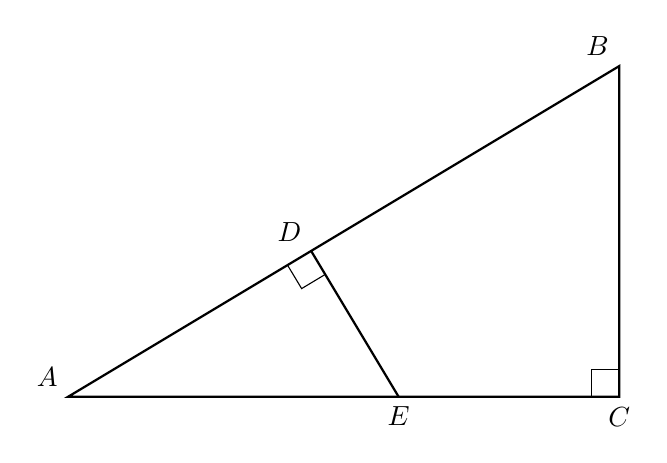
\begin{tikzpicture}[scale=0.7]
    \draw [-, thick] (0,0) node[above left]{$A$}--
    (10,0) node[below]{$C$}--
    (10,6) node[above left]{$B$}--cycle;
    \draw [thick] (6,0)--(4.41,2.65);
    \node at (6,0) [below]{$E$};
    \node at (4.41,2.65) [above left]{$D$};
    \draw (10,0) ++(-0.5,0)--++(0,0.5)--++(0.5,0);
    \draw (4.41,2.65) ++(-59:0.5)--++(-149:0.5)--++(121:0.5);
    %\node at (4, 0) [below]{$12$};
    %\node at (3,2) [above]{$9$};
    %\node at (9, 3) [right]{$10$};
    %\node at (5.5, 1.6) [right]{$6$}; \vspace{1cm}
  \end{tikzpicture}
\end{center} 
If $AB = 9$, $BC = 6$, and $DE = 4$, what is the length of $\overline{AE}$?

\item The diagram below shows $\triangle ABC$, with $\overline{AEB}$, $\overline{ADC}$, and $\angle ACB \cong \angle AED$. $AB=14$, $AD=8$, and $DE=4$. What is the length of $\overline{BC}$?
  \begin{center}
    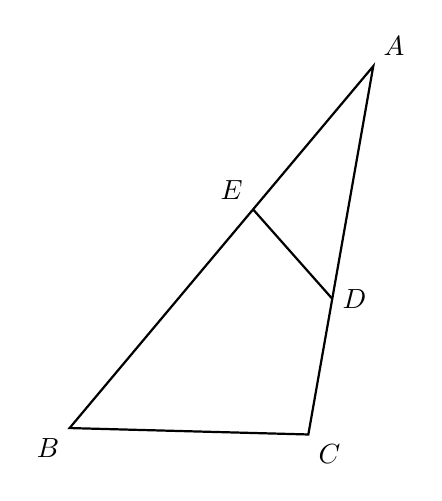
\begin{tikzpicture}[scale=1]
      \draw [thick]
      (0,0) node[above right] {$A$}--
      (230:6) node[below left] {$B$}--
      (260:4.75) node[below right] {$C$}--cycle;
      \draw [thick]
      (230:2.375) node[above left] {$E$}--
      (260:3) node[right] {$D$}--cycle;
    \end{tikzpicture}
  \end{center}

\item Triangle $ADE$ and its midline $\overline{BC}$ are drawn, with $B$ the midpoint of $\overline{AD}$ and $C$ the midpoint of $\overline{AE}$. The two medians $\overline{BE}$ and $\overline{CD}$ are drawn, as shown, intersecting in point $F$, the centroid. Given $BC=8$, $FE=10$. Find $BF$.
  \begin{center}
    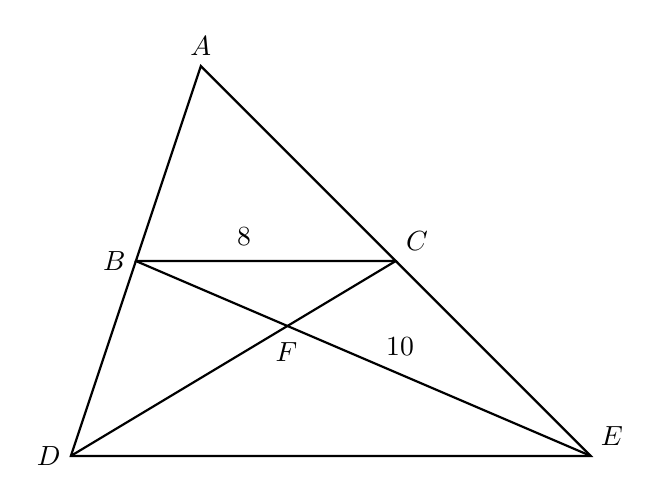
\begin{tikzpicture}[scale=0.55]
      \draw [thick]
      (0.5,1.5)node[left]{$B$}--
      (6.5,1.5)node[above right]{$C$}--
      (2,6)node[above]{$A$}--cycle;
      \draw [thick]
      (0.5,1.5)--
      (-1,-3)node[left]{$D$}--
      (11,-3)node[above right]{$E$}--(6.5,1.5);
      \draw [thick] (0.5,1.5)--(11,-3);
      \draw [thick] (6.5,1.5)--(-1,-3);
      \node at (3,2.5)[below]{$8$};
      \node at (3.5, -0.6)[right]{$F$};
      \node at (6.6, -.9)[above]{$10$};
    \end{tikzpicture}
  \end{center}

\item In trapezoid $ABCD$ below, $\overline{AB} \parallel \overline{CD}$.
\begin{center}
  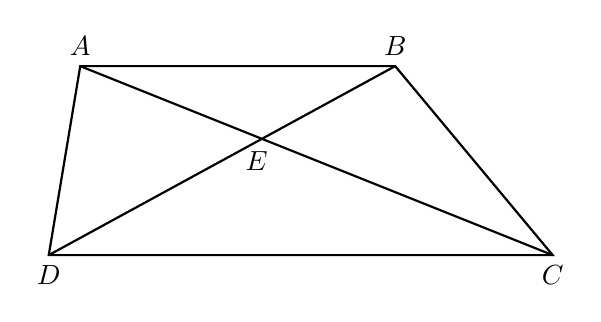
\begin{tikzpicture}[scale=0.8]
    \draw [-, thick] 
      (0,0)node[below]{$D$}--
      (8,0)node[below]{$C$}--
      (5.5,3)node[above]{$B$}--
      (0.5,3)node[above]{$A$}--cycle;
    \draw [-, thick] (0,0)--(5.5,3);
    \draw [-, thick] (0.5,3)--(8,0);
    \node at (3.3, 1.5){$E$};
  \end{tikzpicture}
  \end{center}
If $AE=5.2$, $AC=11.7$, and $CD=10.5$, what is the length of $\overline{AB}$, to \emph{the nearest tenth}?
  
\item In quadrilateral $ABCD$ below, $\overline{AB} \parallel \overline{CD}$, and $E$, $H$, and $F$ are the midpoints of $\overline{AD}$, $\overline{AC}$,  and $\overline{BC}$, respectively.
  \begin{center}
    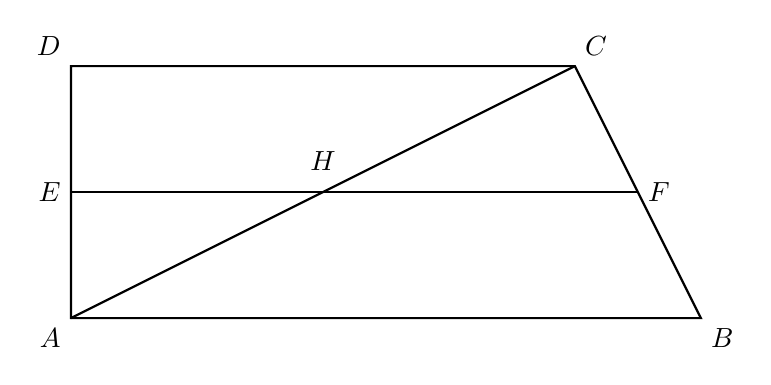
\begin{tikzpicture}[scale=0.8]
      \draw [-, thick] 
        (0,0)node[below left]{$A$}--
        (10,0)node[below right]{$B$}--
        (8,4)node[above right]{$C$}--
        (0,4)node[above left]{$D$}--cycle;
      \draw [-, thick] (0,0)--(8,4);
      \draw [-, thick] (0,2)node[left]{$E$}--(9,2)node[right]{$F$};
      \node at (4,2.5){$H$};
    \end{tikzpicture}
    \end{center}
  If $AB=24$, $CD=18$, and $AH=10$, then what is $FH$?
  
\newpage
\subsubsection*{Similarity (altitude of a right triangle)}
\item Given right triangle $ABC$ with a right angle at $C$, $m\angle B=61^\circ$. Given right triangle $RST$ with a right angle at $T$, $m\angle R=29^\circ$.
  \begin{center}
    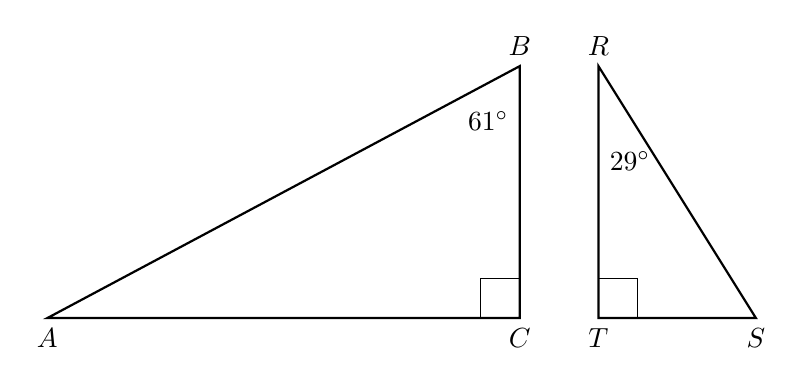
\begin{tikzpicture}[scale=1]
    \draw [thick]
      (0,0)node[below]{$T$}--
      (2,0)node[below]{$S$}--
      (0,3.2)node[above]{$R$}--cycle;
      \draw (0,0)++(0.5,0)--++(0,0.5)--+(-0.5,0);
    \draw [thick]
      (-7,0)node[below]{$A$}--
      (-1,3.2)node[above]{$B$}--
      (-1,0)node[below]{$C$}--cycle;
      \draw (-1,0)++(-0.5,0)--++(0,0.5)--+(0.5,0);
      \node at (-1.4,2.5){$61^\circ$};
      \node at (0.4,2.0){$29^\circ$};
  \end{tikzpicture}
  \end{center}
Which proportion in relation to $\triangle ABC$ and $\triangle RST$ is \emph{not} correct?
  \begin{multicols}{2}
    \begin{enumerate}
      \item $\displaystyle \frac{AB}{RS} = \frac{RT}{AC}$
      \item $\displaystyle \frac{BC}{ST} = \frac{AB}{RS}$ 
      \item $\displaystyle \frac{BC}{ST} = \frac{AC}{RT}$
      \item $\displaystyle \frac{AB}{AC} = \frac{RS}{RT}$
    \end{enumerate}
  \end{multicols}

\item In the accompanying diagram of right triangle $ABC$, altitude $\overline{BD}$ is drawn to hypotenuse $\overline{AC}$.
  \begin{center}
    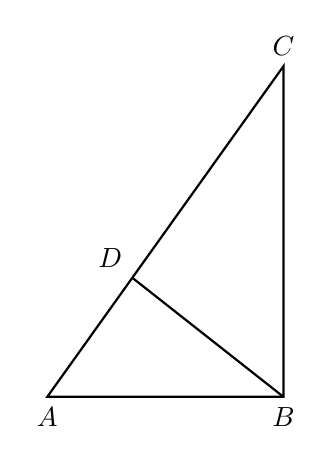
\begin{tikzpicture}[scale=0.6]
    \draw [thick]
    (0,0)node[below]{$A$}--
    (5,0)node[below]{$B$}--
    (5,7)node[above]{$C$}--cycle;
    \draw [thick](1.8,2.52)node[above left]{$D$}--(5,0);
  \end{tikzpicture}
  \end{center}
  Which statement must be true?
  \begin{multicols}{2}
    \begin{enumerate}
      \item $\displaystyle \frac{AD}{AB} = \frac{BC}{AC}$
      \item $\displaystyle \frac{AD}{AB} = \frac{AB}{AC}$ 
      \item $\displaystyle \frac{BD}{BC} = \frac{AB}{AD}$
      \item $\displaystyle \frac{AB}{BC} = \frac{BD}{AC}$
    \end{enumerate}
  \end{multicols}

\newpage
\item In right triangle $RST$ below, altitude $\overline{SV}$ is drawn to hypotenuse $\overline{RT}$.
  \begin{center}
    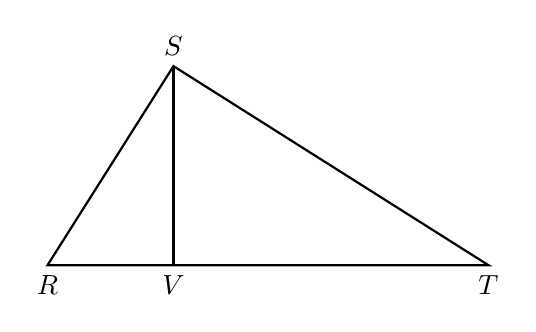
\begin{tikzpicture}[scale=0.8]
    \draw [thick]
    (0,0)node[below]{$R$}--
    (7,0)node[below]{$T$}--
    (2,3.16)node[above]{$S$}--cycle;
    \draw [thick](2,0)node[below]{$V$}--(2,3.16);
  \end{tikzpicture}
  \end{center}
If $RV=4.1$ and $TV=10.2$, what is the length of $\overline{ST}$, to the \emph{nearest tenth}?

\item In the diagram below of right triangle $ABC$, altitude $\overline{BD}$ is drawn to hypotenuse $\overline{AC}$.
  \begin{center}
    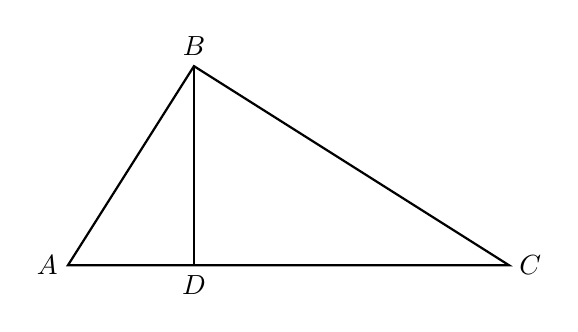
\begin{tikzpicture}[scale=0.8]
    \draw [thick]
    (0,0)node[left]{$A$}--
    (7,0)node[right]{$C$}--
    (2,3.16)node[above]{$B$}--cycle;
    \draw [thick](2,0)node[below]{$D$}--(2,3.16);
  \end{tikzpicture}
  \end{center}
If $BD=4$, $AD=x-6$, and $CD=x$, what is the length of $\overline{CD}$?

\item In the diagram below of right triangle $KMI$, altitude $\overline{IG}$ is drawn to hypotenuse $\overline{KM}$.
  \begin{center}
    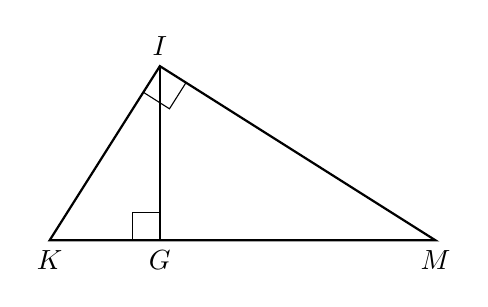
\begin{tikzpicture}[scale=0.7]
    \draw [thick]
    (0,0)node[below]{$K$}--
    (7,0)node[below]{$M$}--
    (2,3.16)node[above]{$I$}--cycle;
    \draw (2,3.16)++(-0.15*2,-0.15*3.16)--++(0.15*3.16,-0.15*2)--+(0.15*2,0.15*3.16);
    \draw [thick](2,0)node[below]{$G$}--(2,3.16);
    \draw (2,0)++(-0.5,0)--++(0,0.5)--+(0.5,0);
  \end{tikzpicture}
  \end{center}
IF $KG=9$ and $IG=12$, what is the length of $\overline{IM}$?

\item Line segment $CD$ is the altitude drawn to hypotenuse in right
triangle $ECF$. If $EC=10$ and $EF=24$, then, to the \emph{nearest
tenth}, $ED$ is what length?

\item In diagram below of right triangle $ABC$, altitude $\overline{BD}$ is drawn.
  \begin{center}
    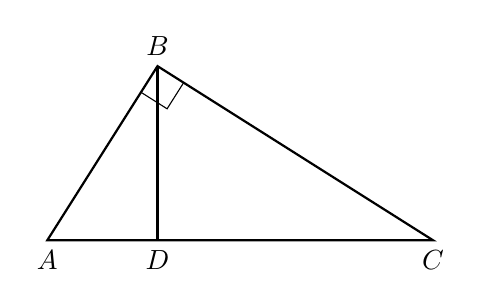
\begin{tikzpicture}[scale=0.7]
    \draw [thick]
    (0,0)node[below]{$A$}--
    (7,0)node[below]{$C$}--
    (2,3.16)node[above]{$B$}--cycle;
    \draw (2,3.16)++(-0.15*2,-0.15*3.16)--++(0.15*3.16,-0.15*2)--+(0.15*2,0.15*3.16);
    \draw [thick](2,0)node[below]{$D$}--(2,3.16);
  \end{tikzpicture}
  \end{center}
Which ratio is always equivalent to $\cos A$?
\begin{multicols}{2}
  \begin{enumerate}
    \item $\displaystyle \frac{AB}{BC}$
    \item $\displaystyle \frac{BD}{BC}$ 
    \item $\displaystyle \frac{BD}{AB}$
    \item $\displaystyle \frac{BC}{AC}$
  \end{enumerate}
\end{multicols}


\newpage
\subsubsection*{Trigonometry}
\item In the diagram below of right triangle $ABC$, $AC=8$, and $AB=17$.
  \begin{center}
    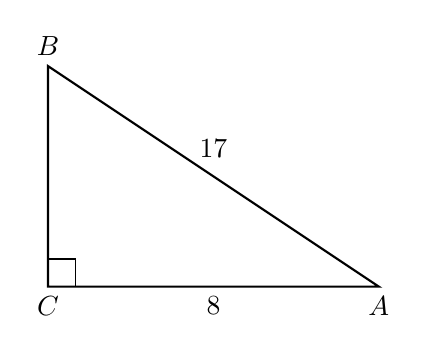
\begin{tikzpicture}[scale=0.7]
    \draw [thick]
      (0,0)node[below]{$A$}--
      (-6,4)node[above]{$B$}--
      (-6,0)node[below]{$C$}--cycle;
      \draw (-6,0)++(0.5,0)--++(0,0.5)--+(-0.5,0);
      \node at (-3,0)[below]{$8$};
      \node at (-3,2.5){$17$};
  \end{tikzpicture}
  \end{center}
Which equation would determine the value of angle $A$?
  \begin{multicols}{2}
    \begin{enumerate}
      \item $\displaystyle \sin A = \frac{8}{17}$
      \item $\displaystyle \tan A = \frac{8}{15}$
      \item $\displaystyle \cos A = \frac{15}{17}$
      \item $\displaystyle \tan A = \frac{15}{8}$
    \end{enumerate}
  \end{multicols}

\item From a point on the ground one-half mile from the base of a historic monument, the angle of elevation to its top is $11.87^\circ$. To the nearest foot, what is the height of the monument? (1 mile = 5280 feet)

\item At a distance of two miles, the angle of elevation to the top of a radio tower is $3.5^\circ$. \\[0.25cm]
What is the height of the tower, to the \emph{nearest foot}? (1 mile = 5280 feet)
  \begin{center}
    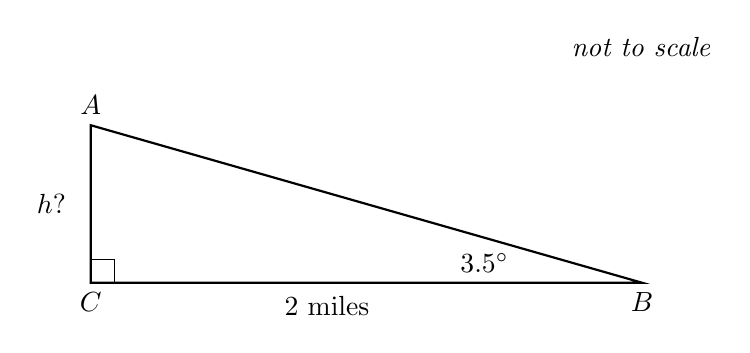
\begin{tikzpicture}[scale=1]
    \draw [thick]
      (0,0)node[below]{$B$}--
      (-7,2)node[above]{$A$}--
      (-7,0)node[below]{$C$}--cycle;
      \draw (-7,0)++(0.3,0)--++(0,0.3)--+(-0.3,0);
      \node at (-7.5,1){$h?$};
      \node at (-2,0.25){$3.5^\circ$};
      \node at (-4,-0.3){2 miles};
      \node at (0,3){\emph{not to scale}};
  \end{tikzpicture}
  \end{center}

\item In right triangle $ABC$, hypotenuse $\overline{AB}$ has a length of 26 cm, and side $\overline{BC}$ has a length of 17.6 cm. What is the measure of angle $B$, to the \emph{nearest degree}?

\item Kayla was cutting right triangles from wood to use for an art project. Two of the right triangles she cut are shown below.
  \begin{center}
    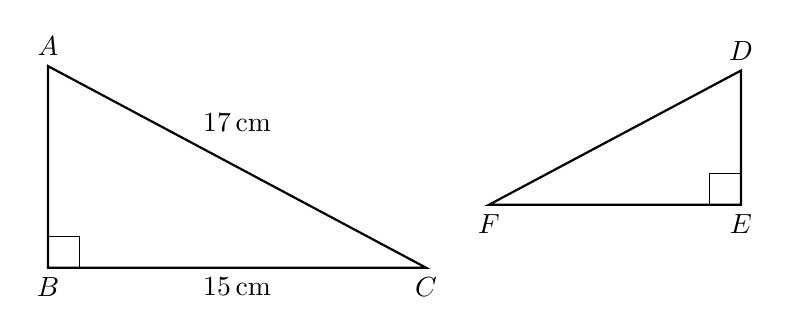
\begin{tikzpicture}[scale=0.8]
    \draw [thick]
      (0,0)node[below]{$F$}--
      (4,0)node[below]{$E$}--
      (4,2.13)node[above]{$D$}--cycle;
      \draw (4,0)++(-0.5,0)--++(0,0.5)--+(0.5,0);
    \draw [thick]
      (-1,-1)node[below]{$C$}--
      (-7,2.2)node[above]{$A$}--
      (-7,-1)node[below]{$B$}--cycle;
      \draw (-7,-1)++(0.5,0)--++(0,0.5)--+(-0.5,0);
      \node at (-4,-1)[below]{$15 \, \rm{cm}$};
      \node at (-4,1.3){$17 \, \rm{cm}$};
  \end{tikzpicture}
  \end{center}
  If $\triangle ABC \sim \triangle DEF$, with right angles B and E, $BC=15$ cm, and $AC=17$ cm, what is the measure of $\angle F$, to the \emph{nearest degree}?

\item In the diagram below of $\triangle HAR$ and $\triangle NTY$, angles $H$ and $N$ are right angles, and $\triangle HAR \sim \triangle NTY$
\begin{center}
  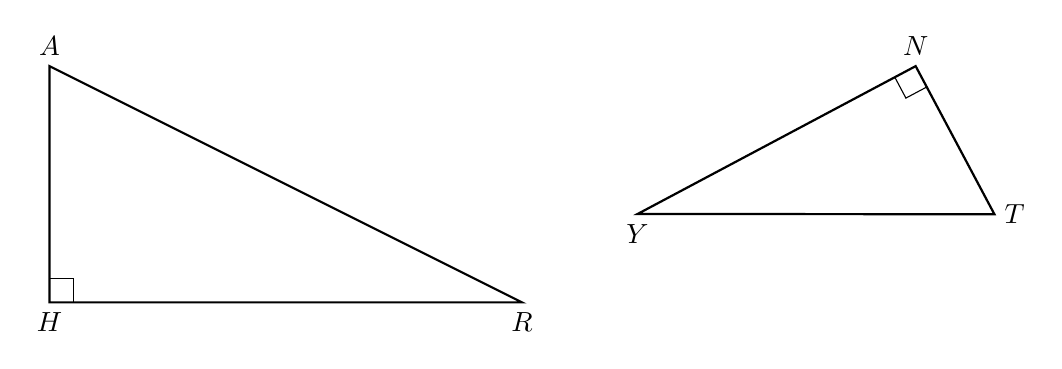
\begin{tikzpicture}[scale=1]
  \draw [thick, xshift=4cm, yshift=2cm, rotate=208]
    (0,0)node[above]{$N$}--
    (4,0)node[below]{$Y$}--
    (0,2.13)node[right]{$T$}--cycle;
    \draw [xshift=4cm, yshift=2cm, rotate=208]
      (0,0)++(0.3,0)--++(0,0.3)--+(-0.3,0);
  \draw [thick]
    (-1,-1)node[below]{$R$}--
    (-7,2)node[above]{$A$}--
    (-7,-1)node[below]{$H$}--cycle;
    \draw (-7,-1)++(0.3,0)--++(0,0.3)--+(-0.3,0);
\end{tikzpicture}
\end{center}
If $AR=13$ and $HR=12$, what is the measure of $\angle Y$, to the \emph{nearest degree}?

\item In the diagram below of right $\triangle ABC$ , $\sin A =\cos B$, $m\angle A = 6x$, and $m\angle B = 3x$. Find $x$.
\begin{center}
  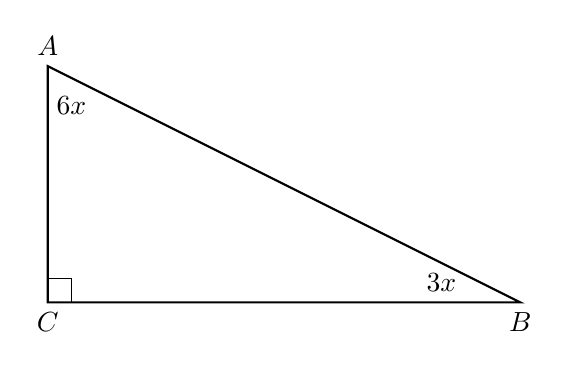
\begin{tikzpicture}[scale=1]
  \draw [thick]
    (-1,-1)node[below]{$B$}--
    (-7,2)node[above]{$A$}--
    (-7,-1)node[below]{$C$}--cycle;
    \draw (-7,-1)++(0.3,0)--++(0,0.3)--+(-0.3,0);
    \node at (-6.7,1.5){$6x$};
    \node at (-2,-0.75){$3x$};
\end{tikzpicture}
\end{center}

\item For the acute angles in a right triangle, $\sin (4x)^\circ =\cos (3x +13)^\circ$. \\
What is the number of degrees in the measure of the smaller angle?

\item In a right triangle, the acute angles have the relationship \\$\sin (2x + 4)=\cos (46)$.\\[0.25cm]
What is the value of $x$?

\item In right triangle $ABC$, $m\angle C=90^\circ$ and $AC \ne BC$. Which trigonometric ratio is equivalent to $\sin B$?
\begin{multicols}{2}
  \begin{enumerate}
    \item $\cos A$
    \item $\cos B$
    \item $\tan A$
    \item $\tan B$
  \end{enumerate}
\end{multicols}

\newpage
\subsubsection*{Circle equations}
\item What is the equation of a circle with center $(5,7)$ and radius $r=3$? 

\item What are the coordinates of the center and the length of the radius of the circle whose equation is $(x-3)^2+y^2=16$?

\item What is the equation of a circle with center $(-3,7)$ and radius $r=4$?

\item The equation of a cirle is $x^2+y^2-2x-14y=-14$. What are the center and radius of the circle?
  
\item The equation of a cirle is $x^2+8x+y^2-12y=144$. What are the coordinates of the center and the length of the radius of the circle?
    \begin{enumerate}
      \item center $(4,-6)$ and radius 12
      \item center $(-4,6)$ and radius 12
      \item center $(4,-6)$ and radius 14
      \item center $(-4,6)$ and radius 14
    \end{enumerate}

\item What is an equation of circle O shown in the graph below?
  \begin{center}
    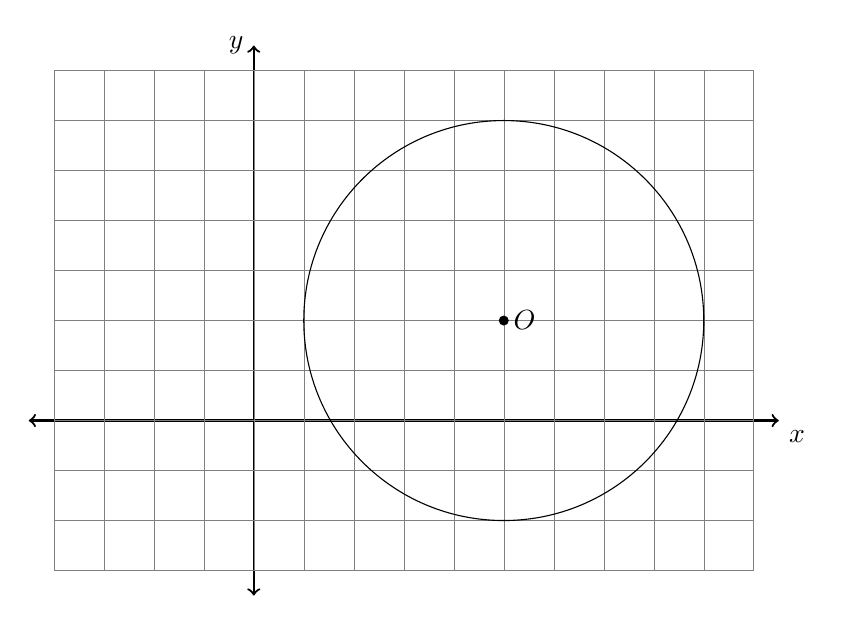
\begin{tikzpicture}[scale=.635]
      \draw [thick, <->] (-4.5,0) -- (10.5,0) node [below right] {$x$};
      \draw [thick, <->] (0,-3.5)--(0,7.5) node [left] {$y$};
      \draw [help lines] (-4,-3) grid (10,7);
      \draw (5,2) circle[radius=4];
        \fill (5,2) circle[radius=.1]node[right]{$O$};
    \end{tikzpicture}
  \end{center}
  \begin{multicols}{2}
    \begin{enumerate}
      \item $x^2+10x+y^2+4y=-13$
      \item $x^2-10x+y^2-4y=-13$
      \item $x^2+10x+y^2+4y=-25$
      \item $x^2-10x+y^2-4y=-25$
    \end{enumerate}
  \end{multicols}

\newpage
\item What are the coordinates of the center and the length of the radius of the circle whose equation is $x^2+y^2=8x-6y+39$?
    \begin{enumerate}
      \item center $(-4,3)$ and radius 64
      \item center $(4,-3)$ and radius 64
      \item center $(-4,3)$ and radius 8
      \item center $(4,-3)$ and radius 8
    \end{enumerate}

\item What is an equation of a circle whose center is (1,4) and diameter is 10?
  \begin{enumerate}
    \item $x^2-2x+y^2-8y=8$
    \item $x^2+2x+y^2+8y=8$
    \item $x^2-2x+y^2-8y=83$
    \item $x^2+2x+y^2+8y=83$
  \end{enumerate}    
     
\item The equation of a cirle is $x^2+y^2+4x-8y=-16$. The statement that best describes circle $O$ is the
    \begin{enumerate}
      \item center is $(2,-4)$ and is tangent to the $x$-axis
      \item center is $(2,-4)$ and is tangent to the $y$-axis
      \item center is $(-2,4)$ and is tangent to the $x$-axis
      \item center is $(-2,4)$ and is tangent to the $y$-axis
    \end{enumerate}

\item What is the equation of a circle whose diameter is $\overline{AB}$ with $A(2,-1)$ and $B(8,7)$?
    \begin{flushright}
      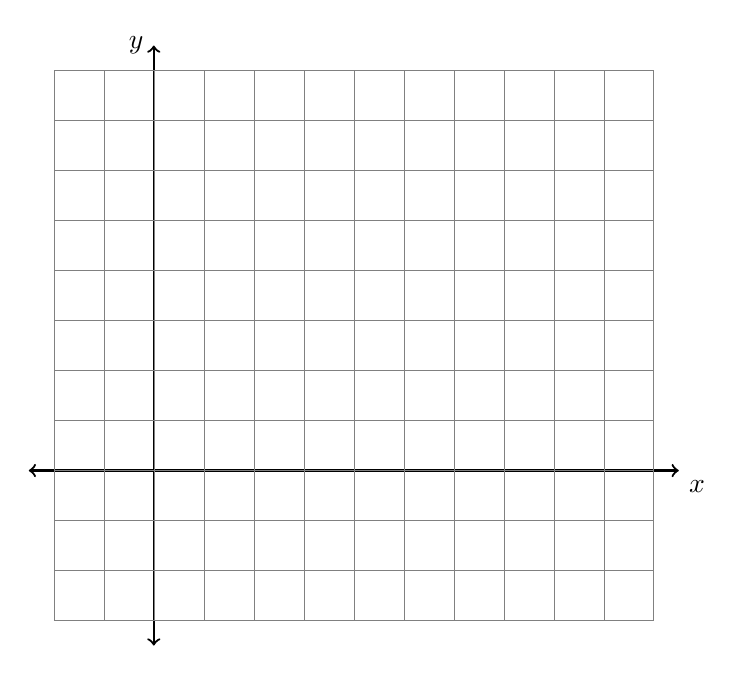
\begin{tikzpicture}[scale=.635]
        \draw [thick, <->] (-2.5,0) -- (10.5,0) node [below right] {$x$};
        \draw [thick, <->] (0,-3.5)--(0,8.5) node [left] {$y$};
        \draw [help lines] (-2,-3) grid (10,8);
      \end{tikzpicture}
    \end{flushright}

\item What are the coordinates of the center and the length of the radius of the circle whose equation is $(x+8)^2+(y-3)^2=4$?

\item What is the equation of a circle with center $(1,-9)$ and radius $r=8$?
  
\item What is an equation of circle O shown in the graph below?
  \begin{center}
    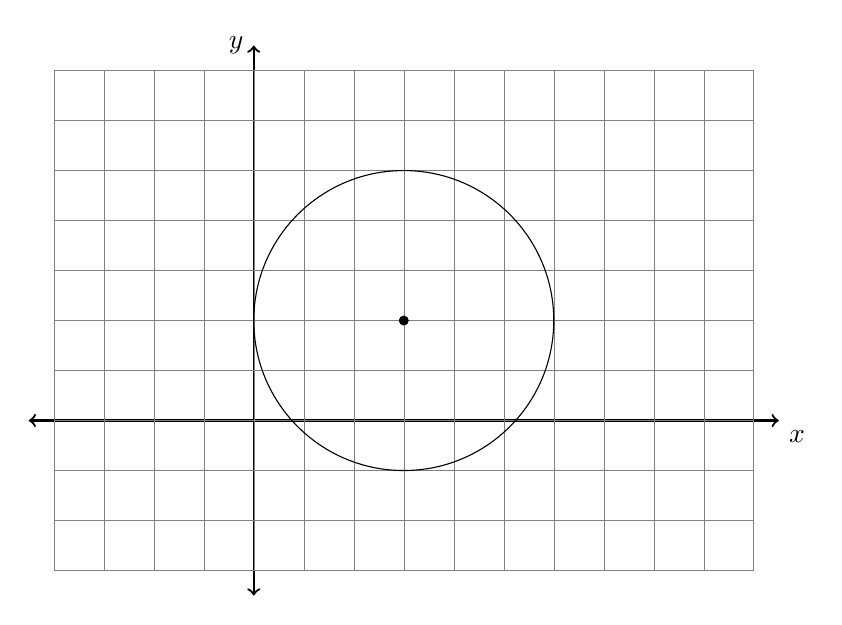
\begin{tikzpicture}[scale=.635]
      \draw [thick, <->] (-4.5,0) -- (10.5,0) node [below right] {$x$};
      \draw [thick, <->] (0,-3.5)--(0,7.5) node [left] {$y$};
      \draw [help lines] (-4,-3) grid (10,7);
      \draw (3,2) circle[radius=3];
        \fill (3,2) circle[radius=.1];
    \end{tikzpicture}
  \end{center}

\item The equation of a cirle is $x^2+y^2-6x+2y=6$. What are the coordinates of the center and the length of the radius of the circle?
  \begin{enumerate}
    \item center $(-3,1)$ and radius 4
    \item center $(3,-1)$ and radius 4
    \item center $(-3,1)$ and radius 16
    \item center $(3,-1)$ and radius 16
  \end{enumerate}

\newpage
\subsubsection*{Chord and sector situations (Similarity)}
\item As shown, circle $O$ has chords $\overline{AD}$ and $\overline{BE}$ intersecting at $C$, and $m \wideparen{AB}=70^\circ$, $m \wideparen{BD}=80^\circ$, $m \wideparen{AE}=100^\circ$, and $m \wideparen{DE}=110^\circ$. $BC=3$, $AC=4$, and $CE=6$.
  \begin{multicols}{2}
  \raggedcolumns
  \begin{flushright}
    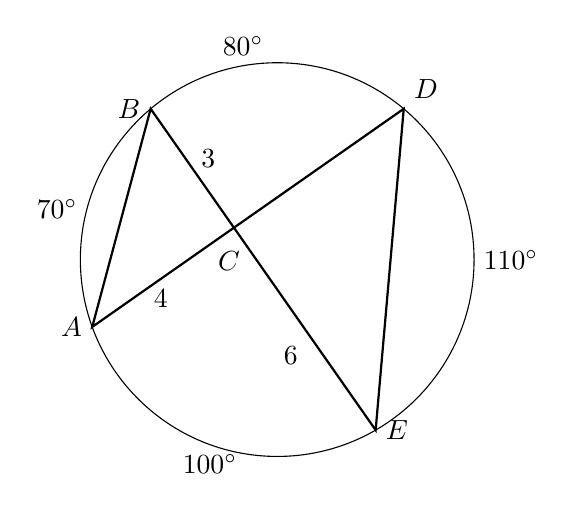
\begin{tikzpicture}[scale=.5]
    \draw (0,0) circle[radius=5];
    \draw [thick]
    (-60:5) node[right] {$E$}--
    (130:5) node[left] {$B$}--
    (200:5) node[left] {$A$}--
    (50:5) node[above right] {$D$}--cycle;
    \draw (160:1.3) node[below] {$C$};
    \draw (120:3.5) node[below] {$3$};
    \draw (190:3) node[below] {$4$};
    \draw (280:2.0) node[below] {$6$};
    \draw (0:5) node[right] {$110^\circ$};
    \draw (100:5) node[above] {$80^\circ$};
    \draw (165:5) node[left] {$70^\circ$};
    \draw (250:5) node[below] {$100^\circ$};
    \end{tikzpicture}
  \end{flushright}
  \begin{enumerate}
    \item Write down the measure of angles $\angle B$ and $\angle D$. \vspace{0.5cm}
    \item Write down the measure of angles $\angle A$ and $\angle E$. \vspace{0.5cm}
    \item Find the measures of the two angles at $C$. \vspace{1.5cm}
    \item Find the scale factor and $CD$.
    \end{enumerate}
  \end{multicols}

  \item Circle $O$ has chords $\overline{AD}$ and $\overline{BE}$ intersecting at $C$, as shown. Find $AC$.
  \begin{center}
    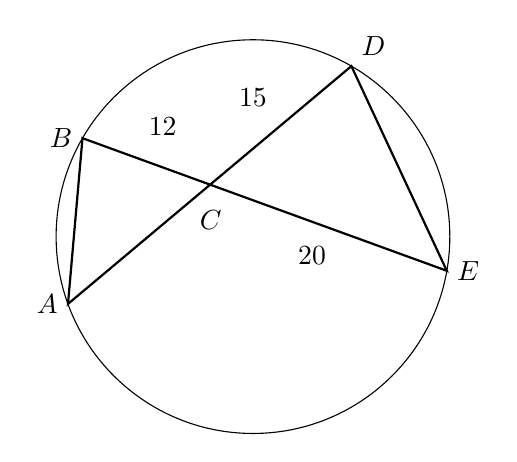
\begin{tikzpicture}[scale=0.5]
     \draw (0,0) circle[radius=5];
     \draw [thick]
     (-10:5) node[right] {$E$}--
     (150:5) node[left] {$B$}--
     (200:5) node[left] {$A$}--
     (60:5) node[above right] {$D$}--cycle;
     \draw (140:1.4) node[below] {$C$};
     \draw (125:4) node[below] {$12$};
     \draw (90:4) node[below] {$15$};
     \draw (0:1.5) node[below] {$20$};
    \end{tikzpicture}
  \end{center}

\item In the diagram below of circle $O$, chords  $\overline{AB}$ and $\overline{CD}$ intersect at $E$.
\begin{center}
  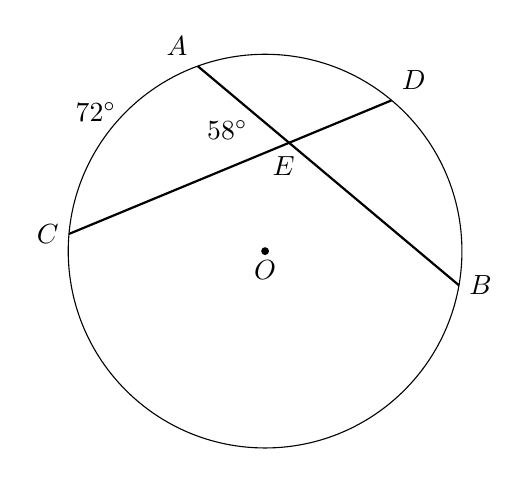
\begin{tikzpicture}[scale=0.5]
   \draw (0,0) circle[radius=5];
   \draw [thick]
   (-10:5) node[right] {$B$}--
   (110:5) node[above left] {$A$};
   \draw [thick] (175:5) node[left] {$C$}--
   (50:5) node[above right] {$D$};
   \draw (80:2.7) node[below] {$E$};
   \fill (0,0) circle[radius=0.1] node[below] {$O$};
   \draw (135:5) node[left] {$72^\circ$};
   \draw (105:3.7) node[below] {$58^\circ$};
  \end{tikzpicture}
\end{center}
If $\textup{m}\wideparen{AC}=72^\circ$ and m$\angle AEC = 58^\circ$, how many degrees are in m$\wideparen{DB}$?

\item In the diagram below, secants $\overline{RST}$ and $\overline{RQP}$, drawn from point $R$, intersect circle $O$ at $S$, $T$, $Q$, and $P$.
\begin{center}
  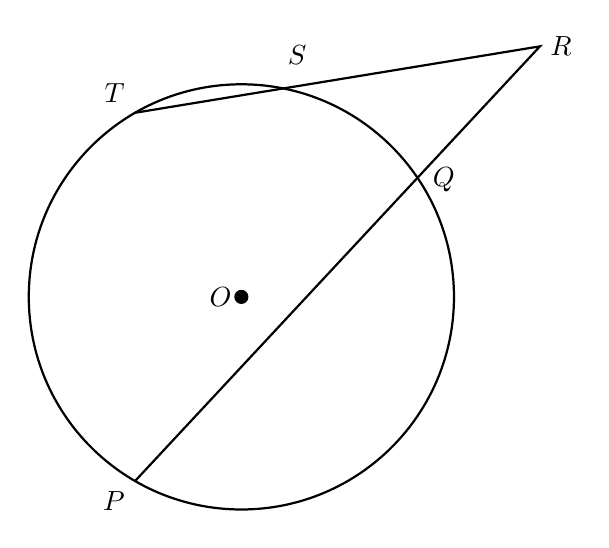
\begin{tikzpicture}[scale=0.9]
    \draw [thick] (0,0) circle[radius=3];
    \fill (0,0) circle[radius=0.1]node[left]{$O$};
    \draw [thick] (120:3)node[above left]{$T$}--
      (40:5.5)node[right]{$R$}--
      (-120:3)node[below left]{$P$};
    \node at (77:3.5){$S$};
    \node at (30:3.3){$Q$};
  \end{tikzpicture}
\end{center}
If $RS=6$, $ST=4$, and $RP=15$, what is the length of $\overline{RQ}$?

\item The secants $\overline{ABC}$ and $\overline{ADE}$ intersect the circle $O$, as shown in the diagram. \\Given $m \wideparen{BD}=36^\circ$ and $m \wideparen{CE}=138^\circ$.
  \begin{enumerate}
    \item Find the $m\angle CDE$, $m\angle CBE$.
    \item Find the $m\angle C$, $m\angle E$.
    \item Find the $m\angle A$.
    \item Two similar triangles are shown. Write a similarity statement, listing the triangles' vertices in corresponding order.
  \end{enumerate}
  \begin{center}
  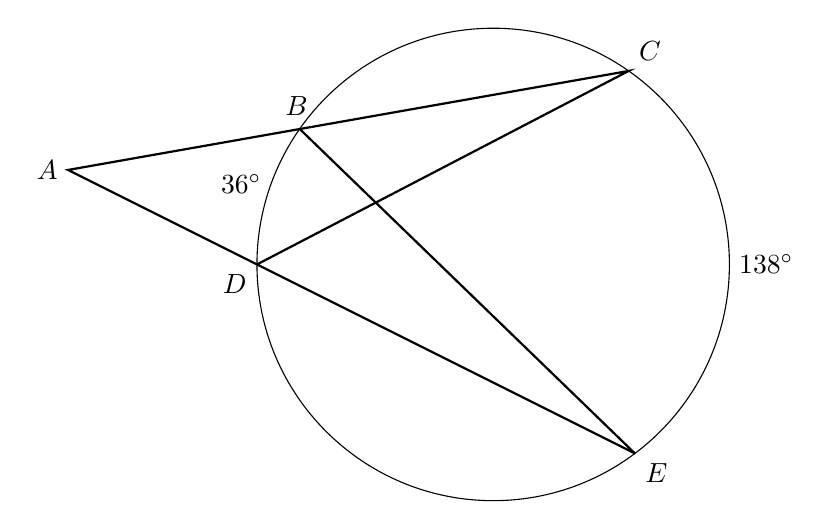
\begin{tikzpicture}[scale=.6]
    \draw (0,0) circle[radius=5];
    \draw [thick]
    (3,-4) node[below right] {$E$}--
    (-5,0) node[below left] {$D$}--
    (-9,2) node[left] {$A$}--
    (55:5) node[above right] {$C$}--
    (-5,0);
    \draw [thick] (3,-4)--(145:5);
    \draw (138:5) node[left] {$B$};
    \draw (0:5) node[right] {$138^\circ$};
    \draw (160:5) node[left] {$36^\circ$};
  \end{tikzpicture}
  \end{center}

\item In the diagram below of circle $O$, secant $\overline{ABC}$ and tangent $\overline{AD}$ are drawn.
\begin{center}
  \begin{tikzpicture}[scale=0.8]
    \draw (0,0) circle[radius=3];
    \fill (0,0) circle[radius=0.1] node[left]{$O$};
    \draw [thick, ->] (150:3) node[above left] {$C$}--
      (20:9) node[right]{$A$}--(-92:4);
    \node at (50:3.3){$B$};
    \node at (-50:3.3){$D$};
  \end{tikzpicture}
\end{center}
If $CA=12.5$ and $CB=4.5$, determine and state the length of $\overline{DA}$.

\item \textbf{External lines:} Circle with center at point $O$, at right.
\begin{multicols}{2}
  \begin{itemize}
    \item Secant $\overline{FGH}$
    \item Radius $\overline{OJ}$
    \item Tangent $\overline{FJK}$
    \item Point of tangency $J$
    \item Note: $\overline{OJ} \perp \overline{FJK}$
  \end{itemize}
  \begin{tikzpicture}[scale=0.6, rotate=-20]
    \draw (0,0) circle[radius=3];
    \draw [thick, ->] (-7,-3) node[above] {$F$}--(4,-3) node[below left] {$K$};
    \draw [thick] (-7,-3)--(72:3) node[above right] {$H$};
    \draw [dashed] (0,-3) node[below] {$J$}--(0,0);
    \fill (0,0) circle[radius=0.1] node[left]{$O$};
    \fill (0,-3) circle[radius=0.1];
    \draw (0,-3) ++(0.5,0)-- ++(0,0.5)--++(-0.5,0);
    \draw (170:3.8) node[below] {$G$};
  \end{tikzpicture}
  \end{multicols}
  
\newpage
\subsubsection*{Analytic geometry}
\item Triangle $DAN$ is graphed on the set of axes below. The vertices of $DAN$ have coordinates $D(-6,-1)$, $A(6,3)$, and $N(-3,10)$.
\begin{center}
  \begin{tikzpicture}[scale=.48]
    \draw [help lines] (-10,-3) grid (10,10);
    \draw [thick, <->] (-10.4,0) -- (10.4,0) node [below right] {$x$};
    \draw [thick, <->] (0,-3.4)--(0,10.4) node [left] {$y$};
    \draw [thick] 
      (-6,-1)node[below left]{$D$}--
      (6,3)node[right]{$A$}--
      (-3,10)node[above]{$N$}--cycle;
  \end{tikzpicture}
\end{center}
What is the area of $\triangle DAN$?

\item In the diagram below, $\triangle ABC$, altitude $\overline{CG}$, and median $\overline{CM}$ are drawn.
\begin{center}
  \begin{tikzpicture}[scale=.48]
    \draw [help lines] (-6,-5) grid (10,9);
    \draw [thick, <->] (-6.4,0) -- (10.4,0) node [below right] {$x$};
    \draw [thick, <->] (0,-5.4)--(0,9.4) node [left] {$y$};
    \draw [thick] 
      (-1,-4)node[below left]{$A$}--
      (7,-3)node[below right]{$C$}--
      (5,8)node[above left]{$B$}--cycle;
    \draw [thick] 
      (1,0)node[above left]{$G$}--
      (7,-3)--
      (2,2)node[left]{$M$};
  \end{tikzpicture}
\end{center}
Which expression represents the area of $\triangle ABC$?
  \begin{multicols}{2}
  \begin{enumerate}
    \item $\displaystyle \frac{(BC)(AC)}{2}$
    \item $\displaystyle \frac{(GC)(BC)}{2}$
    \item $\displaystyle \frac{(CM)(AB)}{2}$
    \item $\displaystyle \frac{(GC)(AB)}{2}$
  \end{enumerate}
  \end{multicols}
  
\item In this problem use the following theorem (copy it at the bottom of the page after your calculations): \\*[0.25cm]
    \emph{A quadrilateral is a parallelogram if and only if it's opposite sides are parallel.}\\*[0.5cm]
    Shown below is quadrilateral $ABCD$, $A(2,-1)$, $B(5,1)$, $C(1,6)$, and $D(-2,4)$. \\*[0.25cm]
    Prove it is a parallelogram by
    \begin{enumerate}
      \item finding the slope of each of the four sides,
      \item stating which sides are parallel,
      \item copying the theorem as your conclusion.
    \end{enumerate}
    \begin{flushright} %4 quadrant regents grid
      \begin{tikzpicture}[scale=.635]
        \draw [help lines] (-5,-4) grid (9,9);
        \draw [thick, <->] (-5.4,0) -- (9.4,0) node [below right] {$x$};
        \draw [thick, <->] (0,-4.4)--(0,9.4) node [left] {$y$};
        \draw [thick] (2,-1) node[below] {$A$}--
        (5,1) node[right] {$B$}--
        (1,6) node[right] {$C$}--
        (-2,4) node[left] {$D$}--cycle;
      \end{tikzpicture}
    \end{flushright}

\item Rhombus $STAR$ has vertices $S(-1,2)$4, $T(2,3)$, $A(3,0)$, and $R(0,-1)$. What is the perimeter of rhombus $STAR$?
    
\item Prove that quadrilateral $ABCD$ is a rectangle by calculating the slope of each side and showing that consecutive sides are perpendicular.

\item Aug 2018 \#35\\
The vertices of quadrilateral MATH have coordinates M(4,2), A(1,-3), T(9,3), and H(6,8). Prove that quadrilateral MATH is a parallelogram.
(scaffold)
  \begin{enumerate}
    \item Find four slopes, starting with: $\displaystyle m_{MA}=\frac{-3-2}{1-4}=$
    \item Make two statements about parallel sides:\\
    $ m_{MA} = m_{TH}$ \emph{iff} $\rule{2cm}{0.015mm} \parallel \rule{2cm}{0.015mm}$ %\vspace{2cm}
    \item Conclusion: $MATH$ is a parallelogram because both pairs of opposite sides are $\rule{3cm}{0.015mm}$
\end{enumerate}

\newpage	
\subsubsection*{Cross sections of solids} %2 problems in 6 exams
  
\item %January 2018
A right hexagonal prism is shown below. A two-dimensional cross section that is perpendicular to the base is taken from the prism.
  \begin{center}
  \includegraphics[scale=0.4]{hex-prism_JA2018.png}
  \end{center}
  Which figure describes the two-dimensional cross section?
  \begin{multicols}{2}
    \begin{enumerate}
      \item rectangle
      \item triangle
      \item pentagon
      \item hexagon
    \end{enumerate}
  \end{multicols}

\item  %August 2018
A right cylinder is cut perpendicular to its base. The shape of the cross section is a
  \begin{multicols}{2}
    \begin{enumerate}
      \item circle
      \item cylinder
      \item rectangle
      \item triangular prism
    \end{enumerate}
  \end{multicols}

\item William is drawing pictures of cross sections of the right circular cone below.
  \begin{center}
    \includegraphics[]{cone.png}
  \end{center}
    Which drawing can \emph{not} be a cross section of a cone?
    \begin{multicols}{2}
    \begin{enumerate}
    \item square
    \item triangle
    \item parabola
    \item ellipse
    \end{enumerate}
    \includegraphics[scale=0.7]{cone-sections.png}
  \end{multicols}

\newpage
\item Which figure can have the same cross section as a sphere?
  \begin{multicols}{2}
    \begin{enumerate}
      \item rectangular prism
      \item pyramid
      \item cone
      \item truncated pyramid
    \end{enumerate}
  \includegraphics[scale=0.5]{solids2.png}
  \end{multicols}

\item The cross section of a regular pyramid contains the altitude of the pyramid. The shape of this cross section is a
  \begin{multicols}{2}
    \begin{enumerate}
      \item circle
      \item square
      \item triangle
      \item rectangle
    \end{enumerate}
  \end{multicols}

\item A two-dimensional cross section is taken of a three-dimensional object. If this cross section is a triangle, what can not be the three-dimensional object?
  \begin{multicols}{2}
    \begin{enumerate}
      \item cylinder
      \item pyramid
      \item cone
      \item rectangular prism
    \end{enumerate}
  \end{multicols}

\item A plane intersects a hexagonal prism. The plane is perpendicular to the base of the prism. Which two-dimensional figure is the cross section of the plane intersecting the prism?
  \begin{multicols}{2}
    \begin{enumerate}
    \item rectangle
    \item triangle
    \item trapezoid
    \item hexagon
    \end{enumerate}
  \end{multicols}


\end{enumerate}
\end{document}
